\begin{figure}[H]
\centering
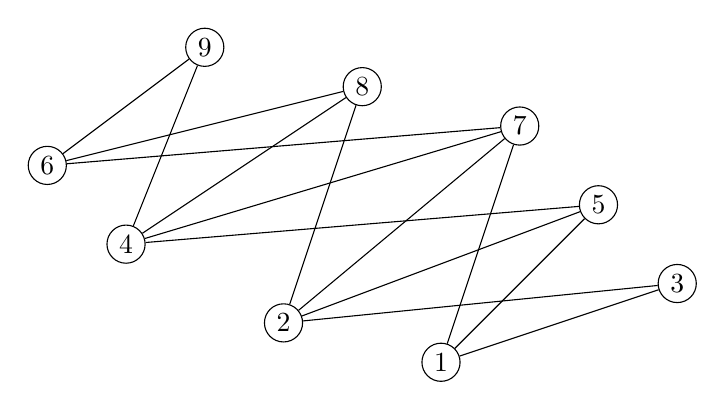
\begin{tikzpicture}
\tikzstyle{vertex}=[draw, circle, inner sep=2pt]
    \node[vertex] (6) at (0,3) {$6$};
    \node[vertex] (4) at (1,2) {$4$};
    \node[vertex] (9) at (2,4.5) {$9$};
    \node[vertex] (2) at (3,1) {$2$};
    \node[vertex] (8) at (4,4) {$8$};
    \node[vertex] (1) at (5,0.5) {$1$};
    \node[vertex] (7) at (6,3.5) {$7$};
    \node[vertex] (5) at (7,2.5) {$5$};
    \node[vertex] (3) at (8,1.5) {$3$};

    \draw (6) -- (9);
    \draw (6) -- (8);
    \draw (6) -- (7);
    
    \draw (4) -- (9);
    \draw (4) -- (8);
    \draw (4) -- (7);
    \draw (4) -- (5);
    
    \draw (2) -- (8);
    \draw (2) -- (7);
    \draw (2) -- (5);
    \draw (2) -- (3);
    
    \draw (1) -- (7);
    \draw (1) -- (5);
    \draw (1) -- (3);
    
\end{tikzpicture}
\label{fig:3n-compgraph}
\caption{A subset close to a $\Grid_{3 \times 3}$ from some large $\CGrid$ using only vertex deletion.}
\end{figure}